\chapter{Overview of Design and Contributions}
\label{ch:contributions}

We summarise the contributions of this thesis in the following list:

\begin{enumerate}
\item Staged an approach to translating semi-formal and formal specifications into Isabelle with automatic assistance.
\item Built tools to enable this approach.
\item Formalised and proved properties of tools and method.
\item Evaluated method and tools on a convincing set of examples.
\end{enumerate}

\section{Staged an approach to translating semi-formal and formal specifications into Isabelle with automatic assistance.}

Translating specifications into theorem provers has shown to be a great difficult task. Not everyone on the software project team will know how to computerise specifications. The first contribution this thesis presents is a new path to assist in the translating formal specifications into theorem provers. This new path has been designed for individuals who have no or little expertise in the chosen theorem prover. This new path is broken up so that each step in the path checks for some form of correctness of the specification. The checks become more and more rigorous the further one goes a long the path.

Using the methodology of MathLang for mathematics (section \ref{sec:mathlangbackground}), I have created and implemented a step by step way of translating Z specifications into theorem provers with additional checks for correctness along the way. This translation consists of one large framework (executed by a user interface) with many smaller tools to assist the translation. Not only is the translation useful for a novice to translate a Z specification into a theorem prover but it also creates other diagrams and graphs to help with the analysis of a formal system specification.

\begin{figure}[H]
 \begin{center}
 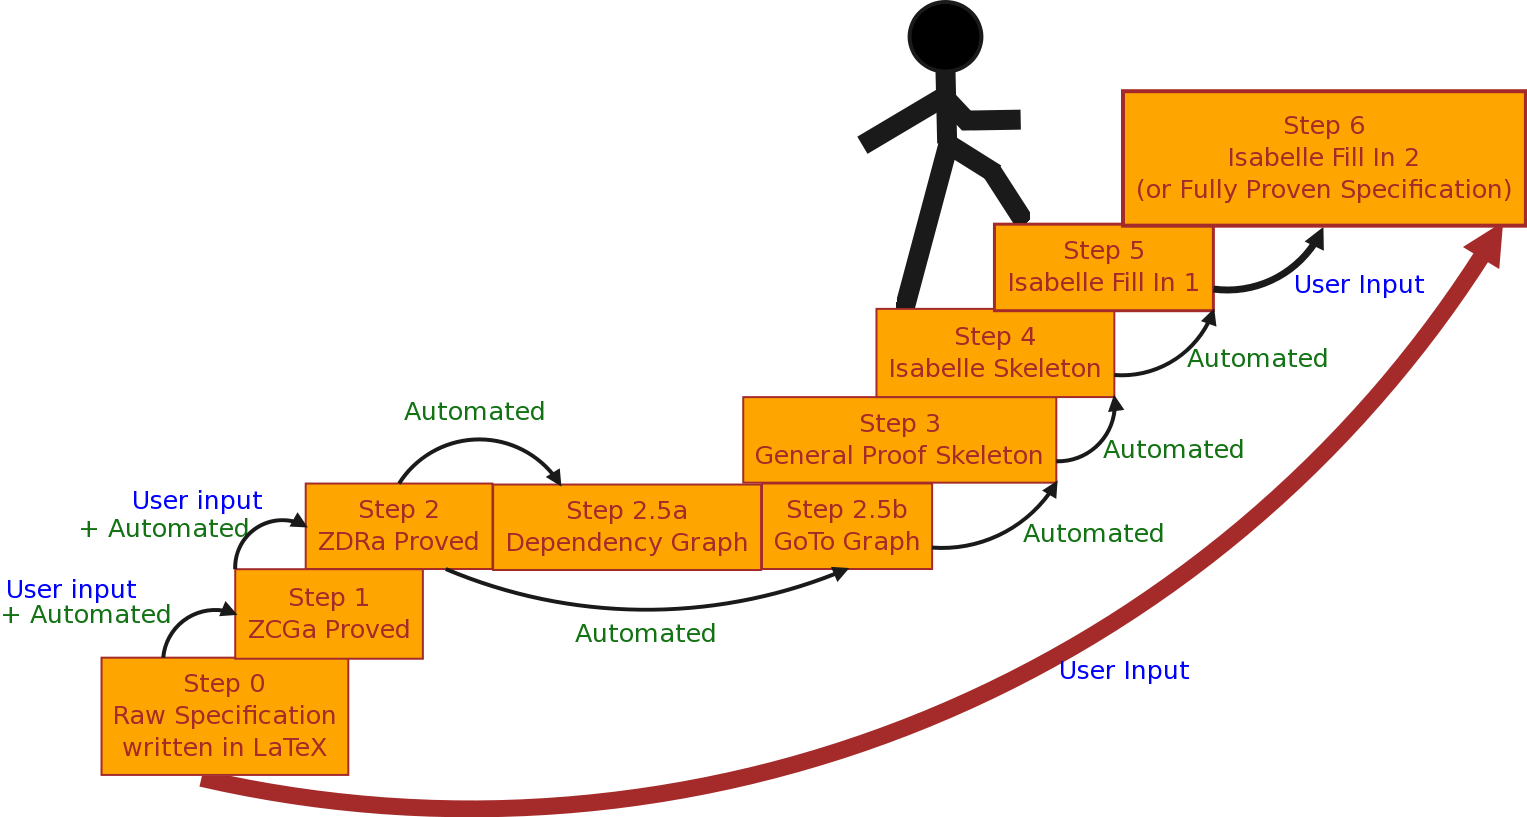
\includegraphics [width=12cm]{Figures/Design/mathlangsteps.png}
 \caption{The steps required to obtain a full proof from a raw specification.}
 \label{fig:steps}
\end{center}
\end{figure} 

The framework is targeted at beginners in theorem proving. The users should have some idea of formal specifications but no or little knowledge of the targetted theorem prover. Figure \ref{fig:steps} shows the outline of the framework. The higher the user goes up the steps the more rigorous the checks for correctness. Step 1 and step 2 are interchangable and can be done in any order. However they both must be completed before moving up to step 3. Step 6 is the highest level of rigour and checks for full correctness in a theorem prover. For this thesis I have chose to translate Z specifications into Isabelle, however this framework is an outline for any formal specification into any theorem prover which could done in the future.

The user doesn't need to go all the way to the top to check for correctness, one advantage of breaking up the translation is that the user gets some level of rigour and can be satisfied with some level of correctness along the way. However the main advantage of breaking up the translation is that the level of expertise needed to check for the correctness of a system specification can be done by someone who has little or no expertise in checking for correctness by a theorem prover.This tool could also aid user in learning theorem proving as it translates their specification and thus they have examples of the syntx used in their theorem prover for their specification. The small black arrows represent the amount of expertise needed for each step. The last step the arrow is slightly thicker as some theorem prover knowledge is needed. However these arrows are still small in comparison to the red thick arrow which represents the translation in one big step.

\section{Built tools to enable this approach (ZCGa, ZDRa Skeletons).}

\section{Formalised and proved properties of tools and method (ZDRa and skeletons).}

\section{Evaluated method and tools on a convincing set of examples.}

%Layout of contribution sections with a couple of pages on each point
%+ Staged an approach to translating semi-formal and formal specifications into Isabelle with automatic assistance.
%+  Built tools to enable this approach (ZCGa, ZDRa Skeletons).
%+ Formalised and proved properties of tools and method (ZDRa and skeletons).
%+ Evaluated method and tools on a convincing set of examples.




% % % % % % % % % % % % % % %OLD CONTRIBUTION SECTION % % % % % % % % % % % % % % % % % % % % % % %
%A summary of contributions is given in the following points:
%
%\begin{itemize}
%\item ZMathLang's \gls{zcga} has been created and implemented.
%
%\begin{itemize}
%
%\item Weak types and weak typing rules have been thoroughly implemented. 
%
%\item A style file has been created to label a specification with \gls{zcga} annotations. This style file also outputs coloured boxes around weak types in the specification so that the user can see the weak types in a clear manner.
%
%\item A weak type checker, which reads the \gls{zcga} annotations and checks they have been implemented.
%
%\item Examples given for various specifications \footnote{The examples for various specifications can be found on \url{http://www.macs.hw.ac.uk/~lb89/zmathlang/examples}}.
%\end{itemize}
%
%\item ZMathLang's \gls{zdra} has been created and implemented. Dependency Graphs and Goto Graphs have been implemented to be automatically generated from the \gls{zdra} annotated document.
%
%\begin{itemize}
%\item Instance names and relations have been carefully realized and added to the \LaTeX{} style file.
%
%\item Relation rules have been outlined.
%
%\item The \gls{zdra} has been implemented to check for the document rhetorical correctness which outputs various warning and error messages.
%
%\item Using directed graphs, dependency and GoTo graphs can be automatically generated from the implementations. Formal aspects of these graphs have also been highlighted.
%
%\item Examples given for various specifications.
%\end{itemize}
%
%\item \gls{gpsa} and Isabelle skeletons have been implemented so they are automatically generated from the \gls{zdra} annotated document.
%
%\begin{itemize}
%
%\item Using the Goto graph a general proof skeleton can be automatically created from the implementation.
%
%\item Using the general proof skeleton an Isabelle skeleton and a filled in skeleton of the original specification can be automatically generated using the implementation.
%
%\item A formal definition of the \gls{zdra}, Dependency graph and GoTo graph has been given.
%\end{itemize}
%
%\item A gradual computerisation path from Z specifications (BirthdayBook \cite{spiveyreferencemanual}, Vending Machine \cite{pp} and all specifications in Curries \cite{essenceofz}) have been documented. These are the first translations from raw Z specifications to complete proofs done using the \gls{zmath} framework. Out of these translations we get new dependency graphs and proof skeletons for the individual specifications.
%
%\begin{itemize}
%\item Clear and concise translation paths from various Z specifications into \gls{zcga} annotated and checked documents, \gls{zdra} annotated and check documents.
%
%\item Dependency graphs, GoTo Graphs and general proof skeletons are generated for all example specifications.
%
%\item Isabelle skeletons automatically generated and filled in for all example specifications.
%
%\item Safety property's and lemma's added to example specifications and proved.
%\end{itemize}
%
%\end{itemize}

% % % % % % % % % % % % % % % % % % % % % % % % % % % % % % % % % % % % % % % % % % % % % % % % % % % % % % % % % % % %